\documentclass{article}

% Language setting
% Replace `english' with e.g. `spanish' to change the document language
\usepackage[english]{babel}

% Set page size and margins
% Replace `letterpaper' with `a4paper' for UK/EU standard size
\usepackage[letterpaper,top=2cm,bottom=2cm,left=3cm,right=3cm,marginparwidth=1.75cm]{geometry}

% Useful packages
\usepackage{amsmath}
\usepackage{amssymb}
\usepackage{amsfonts}
\usepackage{graphicx}
\usepackage[colorlinks=true, allcolors=blue]{hyperref}

\usepackage{natbib}

\title{Evolutionary Pair HMM}
\author{Ian Holmes}

\begin{document}
%\maketitle

\section{Statistical alignment}

\subsection{Expected transition count}

Define some indicator matrices
${\bf J}^{X \to Y}$,
${\bf J}^{\nrightarrow M}$,
${\bf J}^{\rightarrow N}$,
${\bf J}^{M \nrightarrow}$

\begin{eqnarray*}
  J^{X \to Y}_{ij} & = & \left\{ \begin{array}{ll} 1 & \mbox{if $i \in \sigma_X$ and $j \in \sigma_Y$} \\ 0 & \mbox{if $i \notin \sigma_X$ or $j \notin \sigma_Y$} \end{array} \right. \\
  J^{\nrightarrow M}_{ij} & = & \left\{ \begin{array}{ll} 1 & \mbox{if $j \notin \sigma_M$} \\ 0 & \mbox{if $j \in \sigma_M$} \end{array} \right. \\
  J^{\rightarrow N}_{ij} & = & \left\{ \begin{array}{ll} 1 & \mbox{if $j \in \sigma_N$} \\ 0 & \mbox{if $j \notin \sigma_N$} \end{array} \right. \\
  J^{M \nrightarrow}_{ij} & = & \left\{ \begin{array}{ll} 1 & \mbox{if $i \notin \sigma_M$} \\ 0 & \mbox{if $i \in \sigma_N$} \end{array} \right.
\end{eqnarray*}

Let ${\bf U}$ be the transition matrix.

The expected number of transitions of type $X \to Y$
in a path that begins and ends in state 1
is

\[
T_{XY} =
\left(
\left( {\bf I} - {\bf J}^{\nrightarrow M} \circ {\bf U} \right)^{-1}
\left(
     {\bf J}^{X \to Y} \circ
     \left(
     \left( {\bf I} - {\bf J}^{\rightarrow N} \circ {\bf U} \right)^{-1}
          {\bf U}
     \right)
\right)
\left( {\bf I} - {\bf J}^{M \nrightarrow} \circ {\bf U} \right)^{-1}
\right)_{11}
\]

\subsection{Rate of change of expected transition count}

Let ${\bf U}(\theta,t,\delta_t)$ be the transition matrix
of the composite machine $\mathbb{F}(t)\mathbb{G}(\delta_t)$
at time $t$, infinitesimal time increment $\delta_t$, and parameter value $\theta$.
In general this is first-order in $\delta_t$, so it has the form
\[
  {\bf U}(\theta,t,\delta_t) = {\bf U}_0(\theta,t) + {\bf U}_t(\theta,t) \delta_t
  \]

  
  Let $T_{XY}(\theta,t,\delta_t)$ be the corresponding expected number of $X \to Y$ transitions in $\mathbb{FG}$
  between consecutive visits to state 1.

We are interested in
\begin{eqnarray*}
\frac{\partial}{\partial t}T_{XY} & = & \lim_{\delta_t \to 0} \frac{T_{XY}(\theta,t,\delta_t) - T_{XY}(\theta,t,0)}{\delta_t} \\
\frac{\partial^2}{\partial \theta \partial t}T_{XY} & = & \lim_{\delta_\theta \to 0} \lim_{\delta_t \to 0}
\frac{\left(T_{XY}(\theta+\delta_\theta,t,\delta_t) - T_{XY}(\theta+\delta_\theta,t,0)\right) - \left(T_{XY}(\theta,t,\delta_t) - T_{XY}(\theta,t,0)\right)}{\delta_\theta \delta_t}
\end{eqnarray*}

Expand ${\bf U}$ to first order in both $\delta_\theta$ and $\delta_t$
\newcommand\tthetaexpansion[2]{  {#2}_0^{#1}
  + {#2}_\theta^{#1} \delta_\theta
  + {#2}_t^{#1} \delta_t
  + {#2}_{\theta t}^{#1} \delta_\theta \delta_t }
\newcommand\uexpansion{\tthetaexpansion{}{\bf U}}
\newcommand\vexpansion[1]{\tthetaexpansion{#1}{\bf V}}
\[
  {\bf U}(\theta+\delta_\theta,t,\delta_t) = \uexpansion + O(\delta_\theta^2) % + O(\delta_t^2)
\]
where ${\bf U}_0={\bf U}(\theta,t,0)$,
${\bf U}_t=\frac{1}{\delta_t} \left( {\bf U}(\theta,t,\delta_t) - {\bf U}(\theta,t,0) \right)$,
${\bf U}_\theta=\frac{\partial}{\partial \theta} {\bf U}_0$,
${\bf U}_{\theta t}=\frac{\partial}{\partial \theta}  {\bf U}_t$.

We can now expand the matrix inverses.
In general, for ${\bf J} \in \{ {\bf J}^{\nrightarrow M}, {\bf J}^{\rightarrow N}, {\bf J}^{M \nrightarrow} \}$,
\begin{eqnarray*}
  \left( {\bf I} - {\bf J} \circ {\bf U} \right)^{-1}
%  & = &
%  \left( {\bf I} - {\bf J} \circ {\bf U}_0
%  - {\bf J} \circ {\bf U}_\theta \delta_\theta
%  - {\bf J} \circ {\bf U}_t \delta_t
%  - {\bf J} \circ {\bf U}_{\theta t} \delta_\theta \delta_t
%  + O(\delta_\theta^2) + O(\delta_t^2)
%  \right)^{-1} \\
%  & = &
%  \left(
%  \left( {\bf I} - {\bf J} \circ {\bf U}_0 \right)
%  \left( {\bf I}
%  - {\bf V}_0 \left( {\bf J} \circ {\bf U}_\theta \delta_\theta
%  + {\bf J} \circ {\bf U}_t \delta_t
%  + {\bf J} \circ {\bf U}_{\theta t} \delta_\theta \delta_t
%  \right) \right)
%  + O(\delta_\theta^2) + O(\delta_t^2)
%  \right)^{-1} \\
%  & = &
%  \left(
%  \left( {\bf I}
%  + {\bf V}_0 \left( {\bf J} \circ {\bf U}_\theta \delta_\theta
%  + {\bf J} \circ {\bf U}_t \delta_t
%  + {\bf J} \circ {\bf U}_{\theta t} \delta_\theta \delta_t
%  \right)
%  \right) \right)
%  {\bf V}_0
%  + O(\delta_\theta^2) + O(\delta_t^2) \\
%  & = &
%  {\bf V}_0
%  + {\bf V}_0 \left( {\bf J} \circ {\bf U}_\theta \right) {\bf V}_0 \delta_\theta
%  + {\bf V}_0 \left( {\bf J} \circ {\bf U}_t \right) {\bf V}_0 \delta_t
%  + {\bf V}_0 \left( {\bf J} \circ {\bf U}_{\theta t} \right) {\bf V}_0 \delta_\theta \delta_t
%  + O(\delta_\theta^2) + O(\delta_t^2) \\
  & = & \vexpansion{} + O(\delta_\theta^2) + O(\delta_t^2) \\
{\bf V}_0 & = & ({\bf I} - {\bf J} \circ {\bf U}_0)^{-1} \\
{\bf V}_\theta & = & {\bf V}_0 \left( {\bf J} \circ {\bf U}_\theta \right) {\bf V}_0 \\
{\bf V}_t & = & {\bf V}_0 \left( {\bf J} \circ {\bf U}_t \right) {\bf V}_0 \\
{\bf V}_{\theta t} & = & {\bf V}_0 \left( {\bf J} \circ {\bf U}_{\theta t} \right) {\bf V}_0
\end{eqnarray*}

Thus
\begin{eqnarray*}
T_{XY} & = &
\left(
\left( \vexpansion{\nrightarrow M} \right)
\right. \\ & & \quad \times
\left(
     {\bf J}^{X \to Y} \circ
     \left( \left( \vexpansion{\rightarrow N} \right)
     \left( \uexpansion \right) \right)
\right)
 \\ & & \quad \left. \times
 \left( \vexpansion{M \nrightarrow} \right)
\right)_{11}  + O(\delta_\theta^2) + O(\delta_t^2)
\end{eqnarray*}

For convenience define
\[
W_{a,b,c,d} =
\left( {\bf V}^{\nrightarrow M}_a \left( {\bf J}^{X \to Y} \circ \left( {\bf V}^{\rightarrow N}_b {\bf U}_c \right) \right) {\bf V}^{M \nrightarrow}_d \right)_{11}
\]
Examining the coefficients of $\delta_t$ and $\delta_\theta \delta_t$, we see that

\begin{eqnarray*}
  \frac{\partial}{\partial t}T_{XY} & = &
  W_{t,0,0,0} + W_{0,t,0,0} + W_{0,0,t,0} + W_{0,0,0,t}
  \\
  \frac{\partial^2}{\partial \theta \partial t}T_{XY} & = &
  W_{t,\theta,0,0} + W_{t,0,\theta,0} + W_{t,0,0,\theta}
  + W_{\theta,t,0,0} + W_{0,t,\theta,0} + W_{0,t,0,\theta}
  + W_{\theta,0,t,0} + W_{0,\theta,t,0} + W_{0,0,t,\theta}
  \\ & &
  + W_{\theta,0,0,t} + W_{0,\theta,0,t} + W_{0,0,\theta,t}
  + W_{\theta t,0,0,0} + W_{0,\theta t,0,0} + W_{0,0,\theta t,0} + W_{0,0,0,\theta t}
\end{eqnarray*}


\subsection{Runge-Kutta}

Parameters of $\mathbb{F}(t)$ are $\{ T_{XY} \}$.

Parameters of $\mathbb{G}(\delta_t)$ are $\Theta$.

% Runge-Kutta for T_{XY}
% Derivatives of Runge-Kutta w.r.t. \theta_i and T_{XY}


\subsection{Combined model}

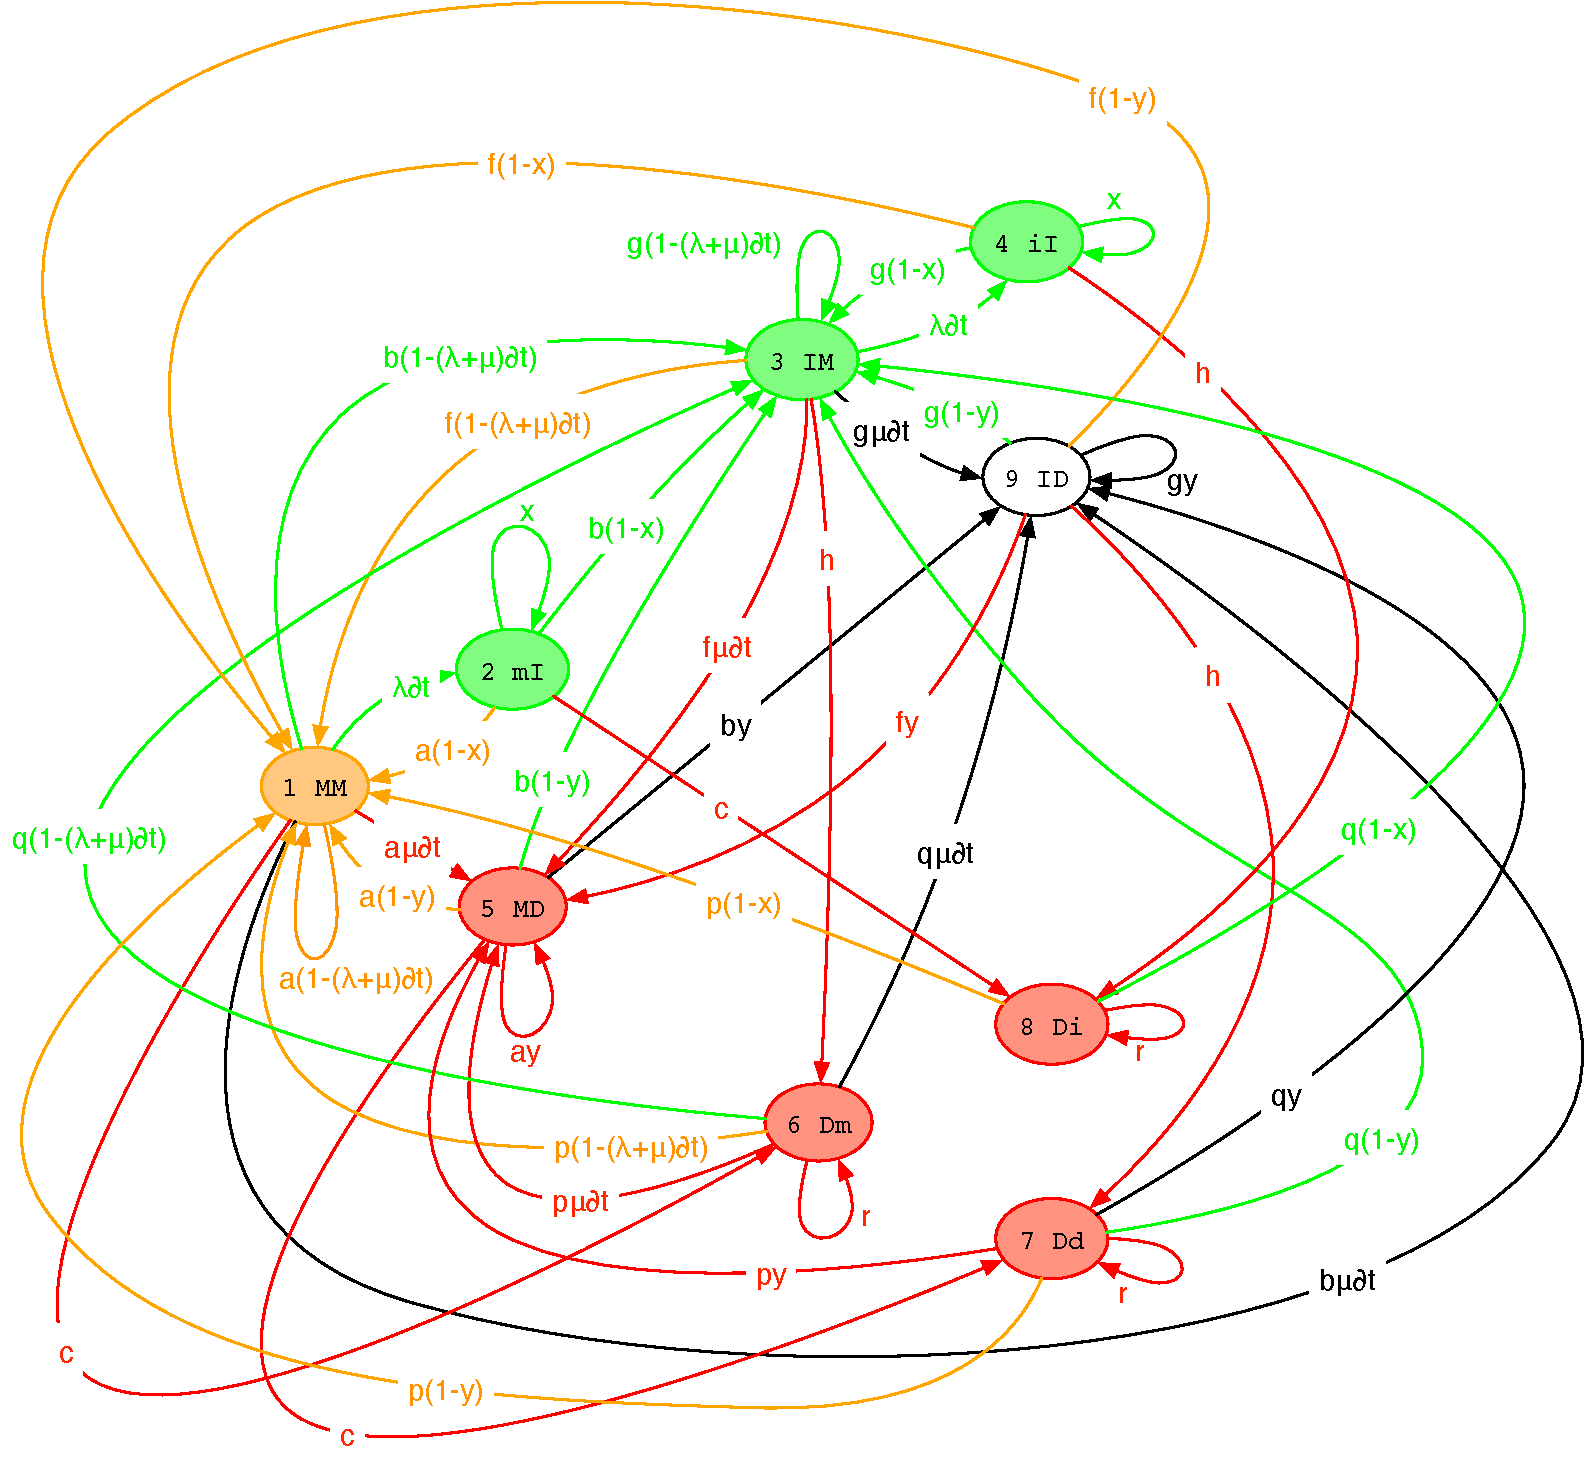
\includegraphics[width=\textwidth]{PairInstant.pdf}

\[
 {\bf U} =
  \left( \begin{array}{ccccccccc}
a (1-(\lambda+\mu) \delta_t) & \lambda \delta_t & b (1-(\lambda+\mu) \delta_t) & 0 & a \mu \delta_t & c & 0 & 0 & b \mu \delta_t \\
a (1-x) & x & b (1-x) & 0 & 0 & 0 & 0 & c & 0 \\
f (1-(\lambda+\mu) \delta_t) & 0 & g (1-(\lambda+\mu) \delta_t) & \lambda \delta_t & f \mu \delta_t & h & 0 & 0 & g \mu \delta_t \\
f (1-x) & 0 & g (1-x) & x & 0 & 0 & 0 & h & 0 \\
a (1-y) & 0 & b (1-y) & 0 & a y & 0 & c & 0 & b y \\
p (1-(\lambda+\mu) \delta_t) & 0 & q (1-(\lambda+\mu) \delta_t) & 0 & p \mu \delta_t & r & 0 & 0 & q \mu \delta_t \\
p (1-y) & 0 & q (1-y) & 0 & p y & 0 & r & 0 & q y \\
p (1-x) & 0 & q (1-x) & 0 & 0 & 0 & 0 & r & 0 \\
f (1-y) & 0 & g (1-y) & 0 & f y & 0 & h & 0 & g y    
  \end{array} \right)
\]

State sets
$\sigma_M=\{1\}$ (orange),
$\sigma_I=\{2,3,4\}$ (green),
$\sigma_D=\{5,6,7,8\}$ (red),
$\sigma_N=\{9\}$ (white).
  
\subsection{General geometric indel model (GGI)}

A sequence ${\cal S}S(t)$ evolves by
substitutions (rate matrix ${\bf Q}$),
deletions (rate $\mu$ per site, extension probability $y$),
and
insertions (rate $\lambda$, extension $x$,
characters $\sim {\bf Q}$'s stationary distribution $\pi$).

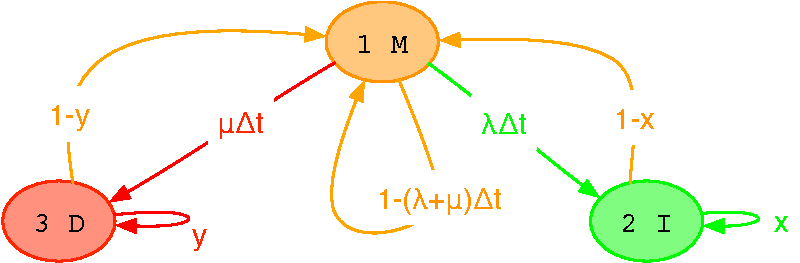
\includegraphics[width=\textwidth]{InstantHMM.pdf}

At equilibrium, sequence length $\sim$ Geometric($\lambda/\mu$). Composition is $\pi$.

If the model is required to be reversible then $\lambda y(1-x) = \mu x(1-y)$.

\subsection{Conditional Pair HMM (transducer) with time-dependent parameters}
Derived in \cite{Holmes2020}.
A Pair HMM whose state path likelihood approximates $P({\cal S}(t)|{\cal S}(0))$

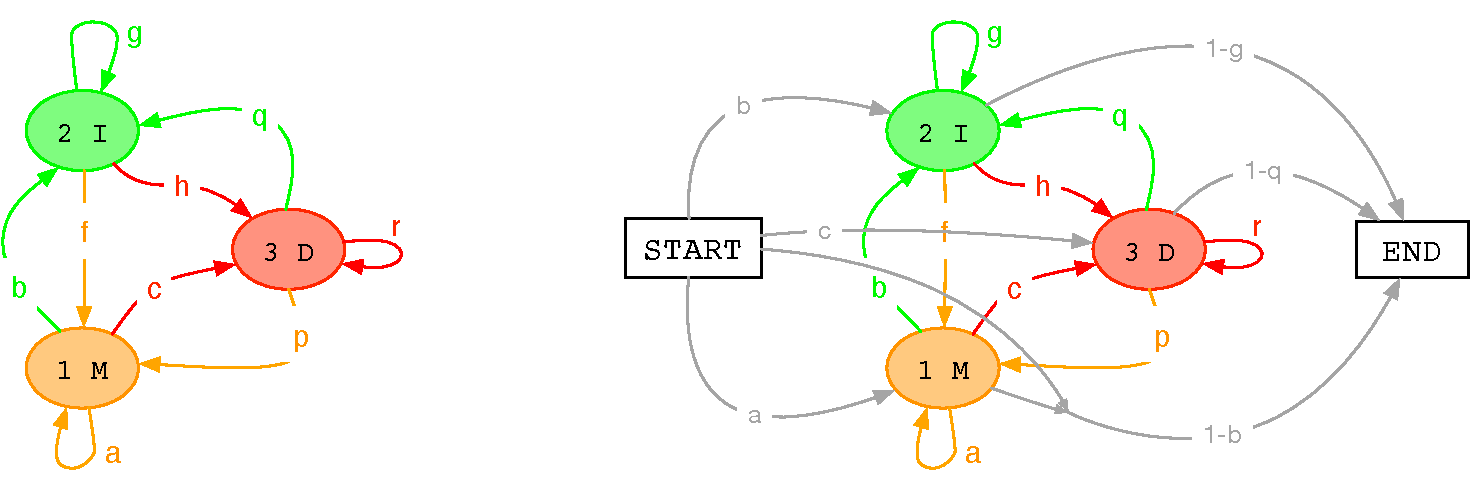
\includegraphics[width=\textwidth]{PairHMM.pdf}

At $t=0$: $a(0)=1$, $f(0)=1-x$, $g(0)=x$, $p(0)=1-y$, $r(0)=y$, and $b(0)=c(0)=h(0)=q(0)=0$.

For $t>0$, % following Holmes (2020)
\begin{eqnarray*}
\begin{bmatrix}
a & b & c \\
f & g & h \\
p & q & r 
\end{bmatrix}
& = &
\begin{bmatrix}
T_{MM} & T_{MI} & 1-T_{MM}-T_{MI} \\
T_{IM}/S_I & (S_I-T_{MI}-T_{DI})/S_I & (T_{MI}+T_{DI}-T_{IM})/S_I \\
(1-T_{MM}-T_{IM})/S_D & T_{DI}/S_D & (S_D+T_{MM}+T_{IM}-T_{DI}-1)/S_D 
\end{bmatrix}
\\
S_I(t) & = & \exp\left(\frac{\lambda t}{1-x}\right)-1 \\
S_D(t) & = & \exp\left(\frac{\mu t}{1-y}\right)-1 \\
T_{ij}(0) & = & \mbox{1 if $i=j=M$, 0 otherwise}
\\
  \frac{d}{dt} T_{MM}(t) & = &
  \mu \frac{b f (1-y)}{1 - g y}-(\lambda +\mu )a
  \nonumber \\
  \frac{d}{dt} T_{MI}(t) & = &
  -\mu \frac{b (1-g)}{1 - g y} + \lambda (1-b)
  \nonumber \\
  \frac{d}{dt} T_{IM}(t) & = &
  \lambda a - \mu \frac{f (1-g) (b (1-r)+c q)}{(1 - g y) (f (1-r)+h p)}
  \nonumber \\
  \frac{d}{dt} T_{DI}(t) & = &
  \mu \frac{(1-g) (b (1-r-h q)+c g q)}{(1-g y) (f (1-r)+h p)}
\end{eqnarray*}

%The $T_{ij}(t)$ may be approximated by Runge-Kutta methods,
%e.g. Dormand-Prince. % \cite{DormandPrince1980}

The substitution matrix for the M state of the Pair HMM is
the matrix exponential $\exp({\bf Q}t)$, for which a Pad\'{e} approximant
or other power series expansion can be used. % \cite{MolerVanLoan2003}

\subsection{Exactly-solved special case (TKF91)}

When $x=y=0$ the model is TKF91 \cite{ThorneEtAl91}
with solution
$
\begin{bmatrix}
a & b & c \\
f & g & h \\
p & q & r 
\end{bmatrix}
=
\begin{bmatrix}
(1-\beta)\alpha & \beta & (1-\beta)(1-\alpha) \\
(1-\beta)\alpha & \beta & (1-\beta)(1-\alpha) \\
(1-\gamma)\alpha & \gamma & (1-\gamma)(1-\alpha)
\end{bmatrix}
$
where
$\alpha = \exp(-\mu t)$,
$\beta = \frac{\lambda \left( \exp(-\lambda t) - \exp(-\mu t) \right)}{\mu \exp(-\lambda t) - \lambda \exp(-\mu t)}$
and
$\gamma = 1 - \frac{\mu \beta}{\lambda (1 - \alpha)}$.



\subsection{Alignment unspecified}

Suppose a prefix list (or tree) of sequences.
Node 1 corresponds to the empty sequence.
Nodes $N>1$ correspond to nonempty sequences ${\cal S}_N$.
Character $\omega_N$ is the last character of ${\cal S}_N$.
The parent node $\psi_N$ corresponds to the longest prefix of ${\cal S}_N$:
removing $\omega_N$ from ${\cal S}_N$ leaves ${\cal S}_{\psi_N}$.

Let $F(i,j,t) = \begin{bmatrix} F_M & F_I & F_D \end{bmatrix}$
be the per-state Forward likelihoods for sequences ${\cal S}_i,{\cal S}_j$.

We seek $F^\dagger(i,j,t) = P({\cal S}(t)={\cal S}_j|{\cal S}(0)={\cal S}_i)$.
The Forward recursions are, for $i>1$ and $j>1$
\begin{eqnarray*}
F(1,1,t) & = & \begin{bmatrix} 1 & 0 & 0 \end{bmatrix}
\\
F(1,j,t) & = &
F(1,\psi_j,t) U_I(\omega_j,t)
\\
F(i,1,t) & = &
F(\psi_i,1,t) U_D(\omega_i,t)
\\
F(i,j,t) & = &
F(\psi_i,\psi_j,t) U_M(\omega_i,\omega_j,t)
+ F(i,\psi_j,t) U_I(\omega_j,t)
+ F(\psi_i,j,t) U_D(\omega_i,t)
\\
F^\dagger(i,j,t) & = & F(i,j,t) \begin{bmatrix}
1-b(t) \\
1-g(t) \\
1-q(t) \end{bmatrix}
\\
U_M(\omega_i,\omega_j,t) & = &
\begin{bmatrix}
a(t) & 0 & 0 \\
f(t) & 0 & 0 \\
p(t) & 0 & 0 
\end{bmatrix}
\exp({\bf Q}t)_{\omega_i \omega_j}
\\
U_I(\omega_j,t) & = &
\begin{bmatrix}
0 & b(t) & 0 \\
0 & g(t) & 0 \\
0 & q(t) & 0 
\end{bmatrix}
\pi_{\omega_j}
\\
U_D(\omega_i,t) & = &
\begin{bmatrix}
0 & 0 & c(t) \\
0 & 0 & h(t) \\
0 & 0 & r(t) 
\end{bmatrix}
\end{eqnarray*}

The time complexity to compute the Forward likelihood is $O(L^2)$,
where $L$ is the sequence length.

\subsection{Alignment specified}

The pairwise alignment of ancestor $i$ and descendant $j$ can be summarized by two lists:
\begin{itemize}
    \item The list $A_M$ of pairs of aligned characters $(\omega,\omega')$ from ancestor ${\cal S}(0)$ and descendant ${\cal S}(t)$;
    \item The list $A_{ID}$ of pairs of unaligned gap sequences $(\delta,\delta')$ that were deleted and inserted in between.
\end{itemize}

The alignment probability, computable in time $O(L)$ (and in practice very fast), is
\[
P(A_M,A_{ID},{\cal S}(t)|{\cal S}(0)) =
\prod_{(\omega,\omega') \in A_M} \exp({\bf Q}t)_{\omega \omega'}
\prod_{(\delta,\delta') \in A_{ID}} G(|\delta|,|\delta'|,t)
\prod_{\omega'\in \delta'} \pi_{\omega'}
\]

where $G(i,j,t)$ is the probability that between the next pair of aligned characters in ${\cal S}(0)$ and ${\cal S}(t)$,
there were $i$ characters deleted from ${\cal S}(0)$ 
and $j$ characters inserted into ${\cal S}(t)$,
with no homology
\begin{eqnarray*}
G(0,0,t) & = & a \\
G(i,0,t) & = & cr^{i-1}p \\
G(0,j,t) & = & bg^{j-1}f \\
G(i,j,t) & = &
g^{j-1} r^{i-1}
\sum_{k=0}^{\min(i,j)}
\left(\frac{hq}{gr}\right)^k
\left[
\binom{i}{k} \binom{j-1}{k} brf
+ \binom{i-1}{k} \binom{j-1}{k} (bhp+cqf)
+ \binom{i-1}{k} \binom{j}{k} cgp
\right]
\end{eqnarray*}
% The unobserved index $k$ counts zig-zags on the Pair HMM state path
% ($D \to I \to D$ or $I \to D \to I$).

\subsection{Phylogenetic alignment}

Both forms of the pairwise likelihood (alignment specified, or unspecified) can be extended to multiple sequences on a phylogeny.
Upgrade $\exp({\bf Q}t)$ to Felsenstein pruning. % \cite{Felsenstein81}.

For the alignment-unspecified form, use automata composition to obtain $N$-sequence HMMs \cite{SilvestreRyanEtAl2020}.
The resulting Forward algorithm is $O(L^N)$.
To ameliorate this, discard all but a few representative sample paths \cite{WestessonEtAl2012},
or use MCMC \cite{RedelingsSuchard2007}.

\bibliographystyle{unsrt}
\bibliography{references}


\end{document}
